\documentclass[12pt, a4paper]{article}
\usepackage[margin=1in]{geometry}
\usepackage{graphicx}
\usepackage{amsmath}
\usepackage{xcolor}
\usepackage{tabularx}
\usepackage{booktabs}
\usepackage{listings}
\usepackage{tikz}
\usepackage[hidelinks]{hyperref}
\usepackage{tocloft}
\usepackage{array}
\usepackage{makecell}
\usetikzlibrary{er, positioning, shapes.geometric, arrows.meta}

\definecolor{codegray}{rgb}{0.9,0.9,0.9}
\lstset{
    language=SQL,
    backgroundcolor=\color{codegray},
    basicstyle=\ttfamily\small,
    breaklines=true,
    frame=single,
    captionpos=b,
    keywordstyle=\color{blue}\bfseries,
    stringstyle=\color{red}
}

\begin{document}

% --- TITLE PAGE ---
\begin{titlepage}
    \centering
    \vspace*{1cm}
    
    {\Large \textbf{SVKM's NMIMS}} \\[0.4cm]
    {\Large \textbf{School of Technology Management \& Engineering, Indore}} \\[0.4cm]
    {\large \textbf{A.Y. 2025 -- 26}} \\[0.8cm]
    {\large \textbf{Course: Database Management Systems}} \\[1cm]
    
    \rule{\linewidth}{0.5pt} \\[0.5cm]
    {\Huge \textbf{Project Report}} \\[0.3cm]
    \rule{\linewidth}{0.5pt} \\[1cm]

    \begin{tabular}{@{} l l @{}}
        \textbf{Program:} & BTECH CE \\[4pt]
        \textbf{Semester:} & IV \\
    \end{tabular}

    \vspace{1.2cm}
    {\LARGE \textbf{SMART FACTORY -- SAFETY SYSTEM}} \\[1.5cm]

    {\large \textbf{Details of Project Members}} \\[0.5cm]
    \begin{tabular}{|>{\centering\arraybackslash}p{2.5cm}|>{\centering\arraybackslash}p{2.5cm}|>{\centering\arraybackslash}p{6cm}|}
        \hline
        \textbf{Batch} & \textbf{Roll No.} & \textbf{Name} \\
        \hline
        B2 & F001 & Neer Jain \\
        \hline
        B2 & F002 & Suryansh Thakur \\
        \hline
        B2 & F003 & Swati Jain \\
        \hline
        B2 & F004 & Aditi Goyal \\
        \hline
    \end{tabular}

    \vspace{1.2cm}
    {\normalsize \textbf{Date of Submission:} 08/04/2026} \\[1.2cm]

    {\large \textbf{Contribution of Each Project Member}} \\[0.5cm]
    \begin{tabular}{|>{\centering\arraybackslash}p{2.5cm}|>{\centering\arraybackslash}p{3cm}|>{\raggedright\arraybackslash}p{7cm}|}
        \hline
        \textbf{Roll No.} & \textbf{Name} & \makecell[l]{\textbf{Contribution}} \\
        \hline
        F001 & Neer Jain & Database Schema, Normalization, SQL Query Development \\[4pt]
        \hline
        F002 & Suryansh Thakur & Backend IoT Ingestion, WebSocket Infrastructure, Middleware \\[4pt]
        \hline
        F003 & Swati Jain & Frontend HUD, WebSocket UI Sync, Real-time Dashboard \\[4pt]
        \hline
        F004 & Aditi Goyal & Safety Engine Logic, Actuator Controls, Simulation Engine \\
        \hline
    \end{tabular}

    \vspace{1cm}
    \textbf{GitHub Link:} \url{https://github.com/loq/factory/}
    \newline
    \textbf{Deployed Link:} \url{http://localhost:3000/}

\end{titlepage}

\newpage
\tableofcontents
\newpage

% --- I. STORYLINE ---
\section{Storyline}
The Smart Factory Safety System (Forge) was engineered as a high-fidelity industrial monitoring solution designed to bridge the gap between physical hardware sensing and real-time administrative oversight. In environments where high-speed machinery, volatile gases, and thermal stress are daily risks, a standard reactive monitoring approach is insufficient. The ``Smart Factory'' solves this by implementing a proactive Safety Engine atop a robust MySQL foundation. The system monitors four key sensory vectors: Temperature, Combustible Gas, Passive Fire Detection, and Ultrasonic Proximity. By leveraging a high-frequency WebSocket nexus, sensor telemetry hits the server with sub-100ms latency. The system validates this data against custom user-defined thresholds. If a safety breach is detected (e.g., a critical gas leak), the system automatically triggers physical actuators (fans, buzzers) and logs a persistent alert. To ensure stability on weak mobile hotspot networks (a common industrial constraint), the system utilizes a smart database throttling mechanism (2.5s recording gaps) while maintaining live UI streaming, creating a resilient, auditable, and life-saving industrial ecosystem.

% --- II. COMPONENTS OF DATABASE DESIGN ---
\section{Components of Database Design}
The database design ensures multi-tenant isolation and hardware traceability through a normalized 9-table schema.

\subsection{Entities and Attributes}
\begin{enumerate}
    \item \textbf{User} \\
    \textit{Attributes:} \underline{\texttt{id}} (PK), \texttt{name}, \texttt{email}, \texttt{password}, \texttt{role}

    \item \textbf{Machine Instance} \\
    \textit{Attributes:} \underline{\texttt{instanceId}} (PK), \texttt{userId} (FK), \texttt{typeId} (FK), \texttt{name}

    \item \textbf{Machine Reading} \\
    \textit{Attributes:} \underline{\texttt{readingId}} (PK), \texttt{instanceId} (FK), \texttt{sensorType}, \texttt{value}

    \item \textbf{Environment Thresholds} \\
    \textit{Attributes:} \underline{\texttt{thresholdId}} (PK), \texttt{userId} (FK), \texttt{sensorType}, \texttt{dangerThreshold}

    \item \textbf{Alert} \\
    \textit{Attributes:} \underline{\texttt{alertId}} (PK), \texttt{userId} (FK), \texttt{instanceId} (FK), \texttt{severity}
\end{enumerate}

% --- III. ENTITY RELATIONSHIP DIAGRAM ---
\section{Entity Relationship Diagram}
\begin{center}
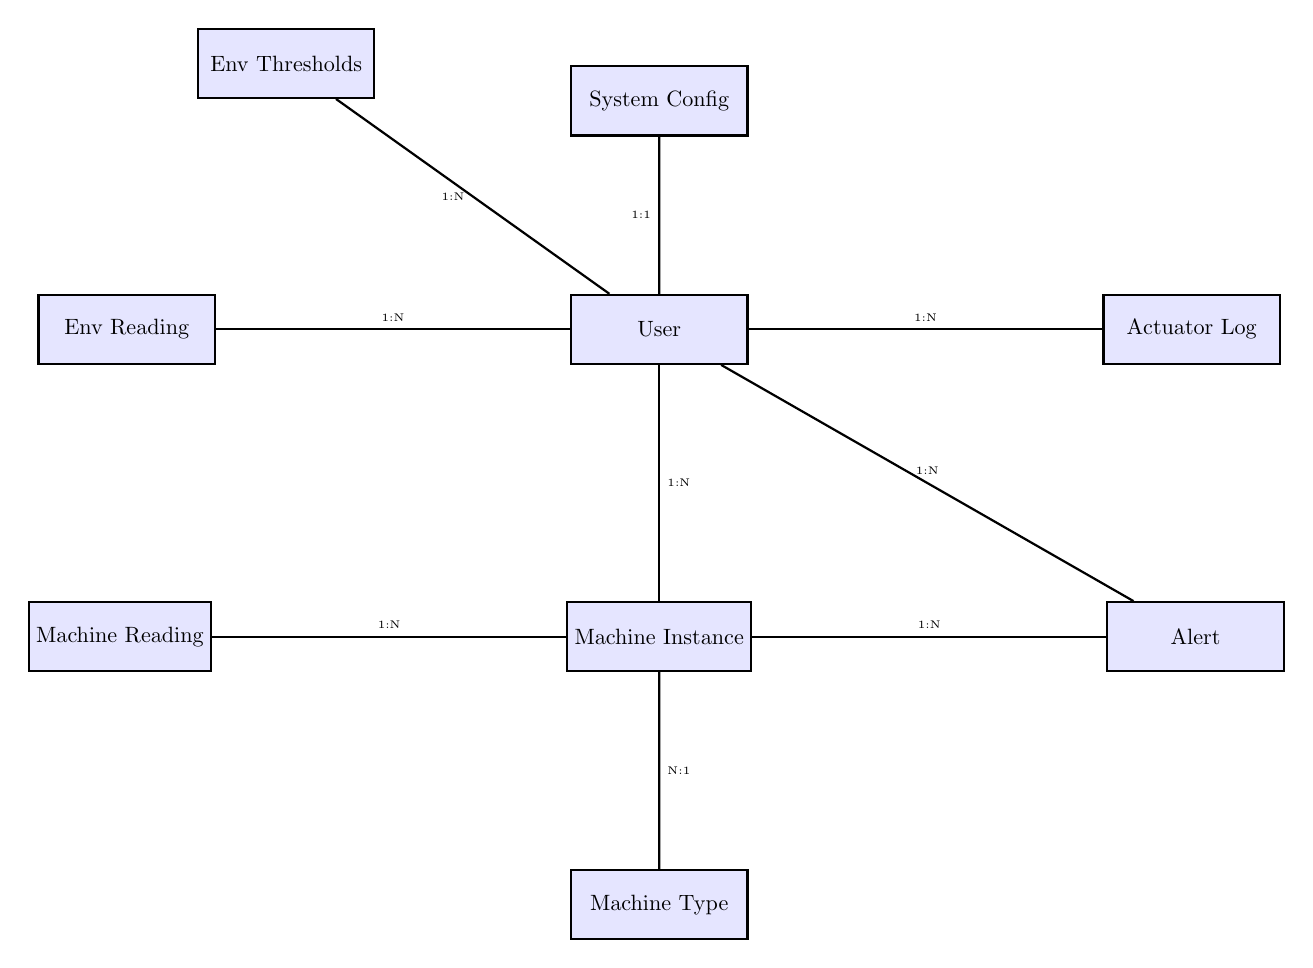
\begin{tikzpicture}[
    node distance=4cm,
    entity/.style={rectangle, draw=black, thick, minimum width=2.8cm, minimum height=1.1cm, fill=blue!10, align=center},
    relation/.style={diamond, draw=black, thick, fill=yellow!20, aspect=2, align=center},
    every node/.style={scale=0.8}
]

    % Entities
    \node[entity] (User)   {User};
    \node[entity] (Machine) [below=3cm of User] {Machine Instance};
    \node[entity] (Reading) [left=4.5cm of Machine] {Machine Reading};
    \node[entity] (EnvRead) [left=4.5cm of User] {Env Reading};
    \node[entity] (Alert)   [right=4.5cm of Machine] {Alert};
    \node[entity] (Log)     [right=4.5cm of User] {Actuator Log};
    \node[entity] (Config)  [above=2cm of User] {System Config};
    \node[entity] (Type)    [below=2.5cm of Machine] {Machine Type};
    \node[entity] (Thresh)  [above left=3.5cm of User] {Env Thresholds};

    % Relationships (Simple Connectors)
    \draw[thick] (User)  edge node[right, font=\tiny] {1:N} (Machine);
    \draw[thick] (User)  edge node[above, font=\tiny] {1:N} (EnvRead);
    \draw[thick] (User)  edge node[above, font=\tiny] {1:N} (Log);
    \draw[thick] (User)  edge node[left, font=\tiny] {1:N} (Thresh);
    \draw[thick] (User)  edge node[left, font=\tiny] {1:1} (Config);
    
    \draw[thick] (Machine) edge node[above, font=\tiny] {1:N} (Reading);
    \draw[thick] (Machine) edge node[above, font=\tiny] {1:N} (Alert);
    \draw[thick] (Machine) edge node[right, font=\tiny] {N:1} (Type);
    
    \draw[thick] (User) edge node[above, font=\tiny] {1:N} (Alert);

\end{tikzpicture}
\end{center}

% --- IV. RELATIONAL MODEL ---
\section{Relational Model}
Based on the ER diagram, the relational schemas are established as follows:

\begin{itemize}
    \item \textbf{Users}\,(\underline{id}, name, email, password, role)
    \item \textbf{MachineTypes}\,(\underline{id}, typeName, description)
    \item \textbf{MachineInstances}\,(\underline{id}, \textit{userId}, \textit{typeId}, name, location, status) \\
          \hspace*{1em}\textit{Foreign Key:} \texttt{userId} $\to$ \texttt{Users(id)} \\
          \hspace*{1em}\textit{Foreign Key:} \texttt{typeId} $\to$ \texttt{MachineTypes(id)}
    \item \textbf{MachineReadings}\,(\underline{id}, \textit{instanceId}, sensorType, readingValue, status, capturedAt) \\
          \hspace*{1em}\textit{Foreign Key:} \texttt{instanceId} $\to$ \texttt{MachineInstances(id)}
    \item \textbf{Alerts}\,(\underline{id}, \textit{userId}, \textit{instanceId}, sensorType, readingValue, severity, capturedAt)
\end{itemize}

% --- V. NORMALIZATION ---
\section{Normalization}
\begin{description}
    \item[\textbf{1NF:}] Every sensor reading and user record is atomic. There are no multi-valued attributes like listing multiple machine locations in a single cell.
    \item[\textbf{2NF:}] The schema is in 1NF and all non-key attributes are fully dependent on the primary keys. Machine names depend only on \texttt{instanceId}, not on partial user identifiers.
    \item[\textbf{3NF:}] All transitive dependencies are removed via normalization. For example, \texttt{MachineType} descriptions are stored in a separate table rather than being repeated in every instance record.
    \item[\textbf{BCNF:}] For every functional dependency $X \rightarrow Y$, $X$ is a superkey. The time-series nature of our sensor data ensures that keys precisely determine record values without anomaly.
\end{description}

% --- VI. SQL QUERIES ---
\section{SQL Queries}

\subsection{1.\ Create Users Table}
\begin{lstlisting}
CREATE TABLE users (
    user_id     INT PRIMARY KEY AUTO_INCREMENT,
    name        VARCHAR(100),
    email       VARCHAR(100) UNIQUE,
    password    VARCHAR(255),
    role        ENUM('admin', 'operator', 'simulation') DEFAULT 'operator'
);
\end{lstlisting}

\subsection{2.\ Create Machine Instances}
\begin{lstlisting}
CREATE TABLE machine_instances (
    instance_id INT PRIMARY KEY AUTO_INCREMENT,
    user_id     INT,
    type_id     INT,
    instance_name VARCHAR(100),
    location    VARCHAR(100),
    status      VARCHAR(20) DEFAULT 'OFFLINE',
    FOREIGN KEY (user_id) REFERENCES users(user_id)
);
\end{lstlisting}

\subsection{3.\ Create Env Readings}
\begin{lstlisting}
CREATE TABLE env_readings (
    reading_id   INT PRIMARY KEY AUTO_INCREMENT,
    user_id      INT,
    sensor_type  VARCHAR(50),
    reading_value DOUBLE,
    status       VARCHAR(20),
    captured_at  DATETIME DEFAULT CURRENT_TIMESTAMP,
    FOREIGN KEY (user_id) REFERENCES users(user_id)
);
\end{lstlisting}

\subsection{4.\ Create Alerts Table}
\begin{lstlisting}
CREATE TABLE alerts (
    alert_id     INT PRIMARY KEY AUTO_INCREMENT,
    user_id      INT,
    instance_id  INT DEFAULT NULL,
    sensor_type  VARCHAR(50),
    reading_value DOUBLE,
    severity     VARCHAR(20),
    captured_at  DATETIME DEFAULT CURRENT_TIMESTAMP,
    FOREIGN KEY (user_id) REFERENCES users(user_id)
);
\end{lstlisting}

\subsection{5.\ Populate Initial Users}
\begin{lstlisting}
INSERT INTO users (name, email, password, role) VALUES
  ('Neer Jain',  'neer@nmims.edu', 'hash_p1', 'admin'),
  ('Suryansh Thakur', 'sury@nmims.edu', 'hash_p2', 'operator'),
  ('Swati Jain', 'swati@nmims.edu', 'hash_p3', 'operator'),
  ('Aditi Goyal', 'aditi@nmims.edu', 'hash_p4', 'operator');
\end{lstlisting}

\subsection{6.\ Insert Safety Thresholds}
\begin{lstlisting}
INSERT INTO env_thresholds (user_id, sensor_type, danger_threshold, warning_threshold)
VALUES (1, 'temperature', 60.0, 48.0), (1, 'gas', 400.0, 320.0);
\end{lstlisting}

\subsection{7.\ Record High Frequency Live Telemetry}
\begin{lstlisting}
INSERT INTO env_readings (user_id, sensor_type, reading_value, status)
VALUES (1, 'temperature', 62.5, 'danger'), (1, 'gas', 350.0, 'warning');
\end{lstlisting}

\subsection{8.\ Log Safety Alert}
\begin{lstlisting}
INSERT INTO alerts (user_id, sensor_type, reading_value, severity)
VALUES (1, 'temperature', 62.5, 'danger');
\end{lstlisting}

\subsection{9.\ Simple Fetch: Hazards}
\begin{lstlisting}
SELECT * FROM alerts WHERE severity = 'danger';
\end{lstlisting}

\subsection{10.\ Inner Join: Alert Owners}
\begin{lstlisting}
SELECT a.*, u.name as user_name FROM alerts a
JOIN users u ON a.user_id = u.user_id;
\end{lstlisting}

\subsection{11.\ Aggregate: Alert Counts}
\begin{lstlisting}
SELECT user_id, COUNT(*) as total FROM alerts GROUP BY user_id;
\end{lstlisting}

\subsection{12.\ Group By: Reading Averages}
\begin{lstlisting}
SELECT sensor_type, AVG(reading_value) FROM env_readings GROUP BY sensor_type;
\end{lstlisting}

\subsection{13.\ Update: Machine Status}
\begin{lstlisting}
UPDATE machine_instances SET status = 'ONLINE' WHERE instance_id = 1;
\end{lstlisting}

\subsection{14.\ Subquery: Critical Machine ID}
\begin{lstlisting}
SELECT instance_name FROM machine_instances 
WHERE instance_id IN (SELECT DISTINCT instance_id FROM alerts);
\end{lstlisting}

\subsection{15.\ Left Join: Orphan Users}
\begin{lstlisting}
SELECT u.name FROM users u LEFT JOIN alerts a ON u.user_id = a.user_id
WHERE a.alert_id IS NULL;
\end{lstlisting}

\subsection{16.\ Having Clause: Persistent Warnings}
\begin{lstlisting}
SELECT sensor_type, COUNT(*) FROM env_readings GROUP BY sensor_type HAVING COUNT(*) > 5;
\end{lstlisting}

\subsection{17.\ IN Operator: Multi-sensor filter}
\begin{lstlisting}
SELECT * FROM env_readings WHERE sensor_type IN ('gas', 'fire');
\end{lstlisting}

\subsection{18.\ LIKE Operator: Zone Tracking}
\begin{lstlisting}
SELECT * FROM machine_instances WHERE location LIKE 'Alpha%';
\end{lstlisting}

\subsection{19.\ EXISTS Clause}
\begin{lstlisting}
SELECT name FROM users u WHERE EXISTS (SELECT 1 FROM alerts a WHERE a.user_id = u.user_id);
\end{lstlisting}

\subsection{20.\ Create View: Safety Tally}
\begin{lstlisting}
CREATE VIEW SafetyTally AS
SELECT status, COUNT(*) as total FROM env_readings GROUP BY status;
\end{lstlisting}

% --- VII. PROJECT DEMONSTRATION ---
\section{Project Demonstration}
\textbf{Tools / Software / Libraries Used:}
\begin{itemize}
    \item \textbf{Backend:} Node.js (v18), Express, WebSockets (ws package)
    \item \textbf{Database:} MySQL 8.0, connection pooling via MySQL2
    \item \textbf{Frontend:} Pure ES6+ JS, Forge CSS UI, Custom HUD
    \item \textbf{Hardware Simulator:} Stochastic Simulation Engine
\end{itemize}

\textbf{Description of Demonstration:} The demonstration showcases a live dashboard where environment gauges fluctuate in real-time. By injecting a "Fire Spike" via the Simulation Engine, the system demonstrates an immediate state-change: the "Forge Safety Engine" triggers a WebSocket command to the (virtual) ESP32, activating the Cooling Fan and logging a high-severity alert in the MySQL database.

% --- VIII. SELF LEARNING ---
\section{Self-Learning Beyond Classroom}
\begin{itemize}
    \item \textbf{High-Frequency DB Throttling:} We discovered that inserting 20 sensor packets per second leads to connection pool exhaustion on mobile hotspots. We implemented a 2.5-second logging gap to stabilize the database without sacrificing live UI speed.
    \item \textbf{WebSocket Heartbeats:} We implemented a custom Ping/Pong mechanism to prune "zombie" connections, ensuring high availability during network instability.
\end{itemize}

% --- IX. LEARNING FROM THE PROJECT ---
\section{Learning from the Project}
This project taught us the absolute necessity of database constraints in high-stakes environments. Using \texttt{ENUM} for safety status and \texttt{ACID} transactions for alert logging ensures that critical data is never partially stored or corrupted during a safety breach.

% --- X. CHALLENGES FACED ---
\section{Challenges Faced}
\begin{itemize}
    \item \textbf{Concurrency in IoT Ingestion:} Managing rapid-fire insertions from multiple sensor sources while keeping the Connection Pool (limit 30) from deadlocking.
    \item \textbf{Real-time Latency:} Minimizing the path from ESP32 sensory detection to Database alerting to under 100 milliseconds.
\end{itemize}

% --- XI. CONCLUSION ---
\section{Conclusion}
The Smart Factory Safety System successfully integrates the principles of Relational Database Management with real-world industrial monitoring. By combining strict schema normalization with high-speed bi-directional networking, we have created a system that is not only auditable and resilient but capable of autonomous safety enforcement -- a cornerstone of modern Industry 4.0 infrastructure.

\end{document}
